\chapter{Rappresentazione simbolica}

Sulla base di quanto introdotto nei capitoli precedenti, vi sono gli elementi per potersi approcciare ad un circuito e tentarne quella che si potrebbe definire la risoluzione, ovvero l'estrapolazione di valori significativi in formato simbolico legati a grandezze specifiche.\graffito{Per l'approccio descritto è necessario che fra le informazioni associate al singolo arco vi sia un parametro che ne descriva la tipologia, ovvero indichi se si tratta di un componente tipo ammettenza, impedenza o nullore} A questo scopo conviene procedere un passo alla volta, descrivendo nei dettagli il comportamento da adottare con circuiti costituiti da soli componenti con rappresentazione ammettenza e transcoduttanze (detti circuiti $RCg_m$), quindi estendendo l'analisi ai componenti con rappresentazione impedenza e infine a tutti quelli che subiscono le imposizioni dovute alla presenza di nullori nei loro modelli equivalenti.

Sarà illustrata inoltre nel prosieguo la tecnica del circuito modificato, la cui utilità consiste nel dare una separazione netta ai componenti dell'espressione finale, così da poterli individuare,  raggruppare ed utilizzare senza difficoltà.

\paragraph{Circuiti $RCg_m$}
Nel caso specifico avremo, da quanto già ampiamente discusso in precedenza, quanto segue:
\begin{itemize}
 \item I componenti bipolari producono, sui due grafi, un ramo fra gli stessi due nodi. Il loro peso, ovvero l'informazione associata a tali rami, è dato dal valore del componente stesso espresso in formato numerico e/o simbolico (laddove presenti).
 \item La transcoduttanza $g_m$ da luogo a un ramo fra i nodi di controllo nel grafo in tensione, mentre nel grafo in corrente introduce un ramo fra i nodi controllati. Da notare che, ai fini del procedimento di assegnamento dell'informazione, in entrambi i grafi il peso del ramo aggiunto è il valore della transcottudanza stessa (nominale e simbolico).
\end{itemize}
Supponiamo di aver ricavato da un circuito $RCg_m$ il grafo in tensione $gV$ ed il grafo in corrente $gI$. Entrambi i grafi avranno $N$ vertici e $M$ archi ed ogni loro albero di copertura conterrà esattamente $N-1$ archi. Supponiamo inoltre che, a partire dai due grafi e applicando uno dei metodi di ricerca degli alberi comuni, si sia ottenuto un insieme di $k$ alberi di copertura comuni:
$$ T = \{ T_1\ldots T_k \}~\mid~ T_i \in \{0\ldots M - 1\}^{N-1}$$
Per cui valga, dalla definizione di albero:
$$ \forall i = 1\ldots k\quad T_i^j \neq T_i^h\quad,\quad\forall j, h \in\{1\ldots N - 1\} ~\mid~ j \neq h $$

Alla luce di tutto ciò avremo che il determinante della matrice delle ammettenze ai nodi può essere calcolato come:
$$
\Delta =
\sum_{i = 1}^k{
  \varepsilon_i\ast\left(\begin{array}{c}
    prodotto~ammettenze~presenti~su~T_i
  \end{array}\right)
}
$$
Dove si abbia come discriminatore del segno:
$$ \varepsilon_i = \pm 1 $$
$$ \varepsilon_i = \left( det\left[ m\{ A_i \} \right] \right)\ast\left( det\left[ m\{ A_v \} \right] \right) $$
Resta da definire chi siano le due matrici $m\{ A_i \}$ e $m\{ A_v \}$. Altro non sono che le matrici d'incidenza ridotte, relative ai due alberi considerati o meglio alla proiezione sui due grafi dell'albero di copertura comune in esame. Poiché la matrice d'incidenza è riducibile ad una matrice quadrata di rango pari a $N-1$ e proprio a causa dell'unimodularità di tale matrice, il determinante sarà dato dai valori $\pm 1$. In realtà potremmo anche avere un determinante pari a $0$ ma tale caso è stato volutamente ignorato poiché, laddove l'evenienza abbia luogo, la matrice delle ammettenze ai nodi non subisce alcun apporto dall'albero comune in esame. Un tale albero può essere semplicemente scartato.

\paragraph{}
Prima di proseguire ulteriormente su questa strada, bisogna aprire una parentesi importante. Prestando attenzione al procedimento di ricerca degli alberi di copertura comuni e quindi a quello di definizione della matrice delle ammettenze ai nodi, si nota come i grafi in corrente e in tensione associati al circuito debbano essere al contempo orientati e non. A motivazione di ciò osserviamo che l'algoritmo di ricerca degli alberi di copertura comuni agisce e parte dal presupposto di operare su un grafo non orientato, infatti la sola idea dell'uso di ponti perde un po' di significato con grafi orientati dove invece avremmo strutture e componenti con definizioni più forti. Allo stesso tempo, è stato appena spiegato come sia utile ricavare le matrici d'incidenza per calcolare quello che si potrebbe definire il segno della matrice delle ammettenze ai nodi.\\
A tal proposito, per onor di cronaca, viene illustrata la semplice soluzione adottata.\\
Facendo un passo indietro, si riscopre la necessità di memorizzare i singoli grafi come liste di archi. Così facendo, per ottimizzare anche l'uso di memoria, si può immagazzinare il singolo arco come fosse orientato, cercando di essere coerenti nel trattare stessi componenti. A questo punto è possibile gestire l'intero grafo come non orientato, considerando che ogni ramo $\left( i, j\right)$ memorizzato definisce implicitamente anche il ramo $\left( j, i\right)$ non memorizzato. Ciò nonostante, per costruzione, il grafo stesso, o meglio i suoi rami portano con loro l'informazione relativa al proprio orientamento, che in questa sede potremmo meglio definire come \textit{orientamento in fase di inserimento}, utilizzabile quando necessario.

\paragraph{Componenti con rappresentazione impedenza}
Volendo allargare la cosa anche a circuiti con componenti non di tipo ammettenza, quali resistenze e induttori, questo è possibile attraverso pochi, semplici passi.

Bisogna però prima fare una premessa introduttiva. Preso un generico albero $T$ su un grafo $G$, si definisce il coalbero di $T$ la foresta $T'$ composta da tutti e soli gli archi non presenti in $T$. In altri termini $T$ e $T'$ definiscono una partizione dell'insieme degli archi presenti nel grafo $G$ in due insiemi più piccoli, ad intersezione nulla, la cui unione definita sui nodi in $G$ dà luogo ancora a $G$ stesso.

L'accenno alla definizione di coalbero è utile per rendere più sintetica l'espressione che segue, definita allo scopo di estendere l'analisi a circuiti con componenti con rappresentazione impedenza. Si modifica la precedente definizione di $\Delta$ in questo modo:
$$
\Delta =
\sum_{i=1}^n{
  \varepsilon_i\ast\left(\begin{array}{c}
    prodotto~ammettenze~presenti~su~T_i\\ \boldsymbol{e~impedenze~presenti~su~T'_i}
  \end{array}\right)
}
$$
Questo è di fatto sufficiente a coprire la presenza di tali elementi.

\paragraph{Circuiti contenenti nullori e generatori controllati non di tipo transcoduttanza}
La rappresentazione dei generatori controllati non di tipo transcoduttanza è, nel caso specifico, ricondotta a modelli equivalenti comprensivi di nullori e generatori controllati di tipo transcoduttanza. Pertanto, poiché quest'ultimi sono già stati presi in considerazione nell'analisi dei circuiti $RCg_m$, in questo frangente è utile analizzare i soli nullori. Su di essi, però, è già stato detto tutto il necessario nei capitoli precedenti. Riassumiamo brevemente in questo paragrafo quanto già detto.

Il nullore comporterebbe, teoricamente, il collasso di una coppia di nodi nel grafo in tensione e di un'altra coppia di nodi nel grafo in corrente, collasso dovuto alla presenza di nullatori e noratori nel proprio schema. Ciò è, intuitivamente, non accettabile nel processo di risoluzione, in tutte le fasi. Una soluzione plausibile, pertanto, consiste nell'inserire un arco per ognuno dei grafi fra i nodi che, altrimenti, subirebbero il collasso, per poi forzare la presenza di tale coppia di archi (o meglio, dell'indice corrispondente) in ognuno degli alberi di copertura comuni. Questo porta ad avere una base comune fra ogni albero individuato, derivante appunto dalla presenza di nullori.

\paragraph{Metodo del circuito modificato}
Quanto definito è sufficiente per ottenere in modo corretto il determinante della matrice $\Delta$ delle ammettenze ai nodi.

Consideriamo allora la matrice dei cofattori. Per la natura di matrice quadrata della matrice $A$ delle ammettenze ai nodi, essa ammette la presenza di un'ulteriore matrice quadrata avente stesso ordine e detta, appunto, matrice dei cofattori. Per la posizione generica $\left( i, j\right)$ vale il valore o cofattore:
$$ cof\left( A, i, j\right) = (-1)^{i+j}\ast det\left[ minore\left( A, i, j\right)\right] $$
Dove per $minore\left( A, i, j\right)$ si intende la matrice (ancora quadrata) ottenuta da $A$ eliminando le righe $i$ e $j$.

Poniamo la massa come nodo $0$. Supponendo adesso di voler eccitare il circuito in esame fra i nodi $i$ e $0$, per poi calcolarne l'uscita fra i terminali $j$ e $0$, possiamo scrivere le formule di trasferimento come segue:
$$ Z_{in} = \frac{V_i}{I_i} = \frac{\Delta_{ii}}{\Delta} $$
$$ \frac{V_o}{I_{in}} = \frac{V_j}{I_i} = \frac{\Delta_{ij}}{\Delta} $$
$$ \frac{V_o}{V_{in}} = \frac{V_j}{V_i} = \frac{\Delta_{ij}}{\Delta_{ii}} $$
Dove valgono le seguenti relazioni:
$$
\begin{array}{c}
 \Delta = determinante~matrice~ammettenze~ai~nodi\\
 \Delta_{ij} = ij_{esimo}~cofattore~matrice~ammettenze~ai~nodi
\end{array}
$$

\begin{figure}
 \centering
 \subfloat[Circuito originale]{\label{fig:circbase}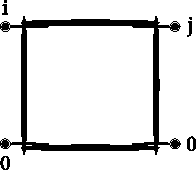
\includegraphics{immagini/circbase.pdf}}
 \hspace{25pt}
 \subfloat[Circuito modificato]{\label{fig:circmod}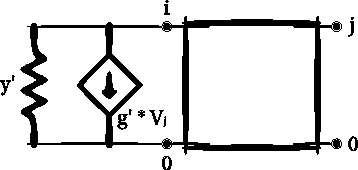
\includegraphics{immagini/circmod.pdf}}
 \caption{Metodo del circuito modificato}
 \label{fig:circmet}
\end{figure}

Sebbene il calcolo illustrato sia a tutti gli effetti corretto, non si può dire che sia allo stesso tempo anche efficace e maneggevole. Qui entra in gioco il metodo del circuito modificato, atto a rendere facilmente recuperabili i dati sensibili coinvolti nell'analisi.

In figura \ref{fig:circmet} è riportato visivamente ciò di cui consiste concretamente questa tecnica. Rifacendosi all'esempio sopra citato, cioè ad una sollecitazione applicata fra i nodi $i$ e $0$ per poi valutarne gli effetti sui terminali $j$ e $0$, si può guardare al circuito come nella forma proposta in figura \ref{fig:circbase}. Aggiungendo quindi fra i due nodi in ingresso un'ammettenza e una transcoduttanza\graffito{Ammettenza e transconduttanza ausiliarie introdurranno nei due grafi archi che dovranno essere marcati con speciali valori per quanto riguarda la loro tipologia, pur rientrando nella categoria delle ammettenze}, quest'ultima legata ai terminali di uscita, si ricava il circuito modificato riportato in figura \ref{fig:circmod}. Il determinante della matrice delle ammettenze per il circuito modificato diventa:
$$ \Delta ' = \Delta + y'\Delta_{ii} + g'\Delta_{ij} $$
Si nota come siano stati di fatto ricavati in modo immediato i cofattori coinvolti nel calcolo dell'impedenza in ingresso, la transimpedenza e la funzione di trasferimento. Sarà adesso possibile procedere senza difficoltà ricercando in $\Delta '$ tutti i valori d'interesse, semplicemente individuando $y'$ e $g'$.
